\chapter{The Governing Equations \label{governingequations}}
The semi-geostrophic equations first introduced by \cite{Eliassen1962}
form the basis of our model for frontogenesis. Widely noted to be more rigorous than the classical quasi-geostrophic equations in their description of the formation of weather fronts 
\cite{Cullen2006a, Hoskins1975}. 
In this chapter a summary of key steps that lead to the Eady model for frontogensis that was developed by Hoskins and Bretherton , 1972, \cite{Hoskins1972} is given. Based on the model for baroclinic instability proposed by Eady, 1949, incorporating a linear stratification in density and a constant vertical shear in the horizontal velocity component. A co-ordinate transform to geostrophic co-ordinates by  \cite{Hoskins1975} 
facilitates the numerical implementation of these equations and subsequent interpretation of results. For the following the main points are summarised from Cullen 2006 \cite{Cullen2006a} in formulating the model to be implemented numerically.
\section{The Semi-Geostrophic Equations \label{SGeqns}} 
\subsection{The 3D Incompressible Boussinesq Equations}
\begin{figure}[h]
	\centering
	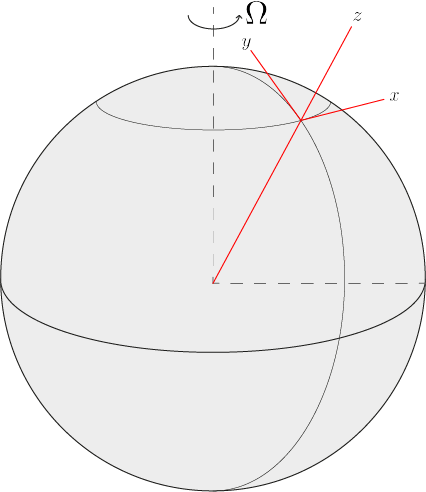
\includegraphics[width=5cm]{background/local_cartesian}
	\caption{Local cartesian co-ordinates $\left(x,y,z\right)$ on Earth}
	\label{fig:localcartesian}
\end{figure}
We begin with the $3$D incompressible Boussinesq equations \ref{3DBous} to describe atmospheric flow. Adopting cartesian co-ordinates $\left(x,y,z\right)$ representing the zonal, meridional and radial directions on the Earth respectively, as shown in \ref{fig:localcartesian}. The corresponding velocity components are $\bm{u}=\left(u,v,w\right)$, with $\rho_0$ representing the constant density and $p$ denoting the pressure.
\begin{equation}
	\begin{aligned}
		\frac{\mathrm{D}u}{\mathrm{D}t}	- fv  &= -\frac{1}{\rho_0}\frac{\partial p}{\partial x}\\
		\frac{\mathrm{D}v}{\mathrm{D}t}	+ fu  &= -\frac{1}{\rho_0}\frac{\partial p}{\partial y}\\
		\frac{\mathrm{D}w}{\mathrm{D}t} &= -\frac{1}{\rho_0}\frac{\partial p}{\partial z} + b\\
		\frac{\mathrm{D} b}{\mathrm{D}t} &= 0\\
		\nabla \cdot \bm{u} &= 0
	\end{aligned}
\label{3DBous}
\end{equation}
Under the Boussinesq assumption that density fluctuations are small, the thermodynamic equation is written as equation (4) in the system above. The buoyancy is characterised by Potential Temperature, $\theta$ as $b = \frac{g\theta}{\theta_0}$. By also introducing the geopotential $\phi = \frac{p}{\rho_0}$, equations \ref{3DBous} are rewritten as
\begin{equation}
	\begin{aligned}
		\frac{\mathrm{D}u}{\mathrm{D}t}	- fv  &= -\frac{\partial \phi}{\partial x}\\
		\frac{\mathrm{D}v}{\mathrm{D}t}	+ fu  &= -\frac{\partial \phi}{\partial y}\\
		\frac{\mathrm{D}w}{\mathrm{D}t} &= -\frac{\partial \phi}{\partial z} + \frac{g\theta}{\theta_0}\\
		\frac{\mathrm{D} \theta}{\mathrm{D}t} &= 0\\
		\nabla \cdot \bm{u} &= 0
	\end{aligned}
\label{3DBousPT}
\end{equation}
where $\theta_0$ and $g$ denote initial potential temperature and acceleration due to gravity respectively. \\
$\frac{\mathrm{D}}{\mathrm{D}t} \equiv \frac{\partial}{\partial t} + u\frac{\partial}{\partial x} + v\frac{\partial}{\partial y} + w\frac{\partial}{\partial z},\qquad$ 
$\nabla \equiv \left(\frac{\partial}{\partial x}, \frac{\partial}{\partial y},\frac{\partial}{\partial z}\right)$ \\
\linebreak
Additionally if the hydrostatic approximation, that vertical acceleration is small compared to gravity, so that, $\frac{\mathrm{D}w}{\mathrm{D}t} = 0$. Then, 
\begin{equation}
	\begin{aligned}
	\frac{\mathrm{D}u}{\mathrm{D}t}	- fv  &= -\frac{\partial \phi}{\partial x}\\
	\frac{\mathrm{D}v}{\mathrm{D}t}	+ fu  &= -\frac{\partial \phi}{\partial y}\\
	-\frac{\partial \phi}{\partial z} + \frac{g\theta}{\theta_0} &= 0\\
	\frac{\mathrm{D} \theta}{\mathrm{D}t} &= 0\\
	\nabla \cdot \bm{u} &= 0
	\end{aligned}
	\label{3DBousPThydro}
\end{equation}
\subsection{The Vertical Slice Model}
To facilitate the study of frontogenesis a vertical slice model is introduced. In this report the vertical slice is defined as the $\left(x-z\right)$ plane. The domain considered is defined as, $\Gamma := [-L,L] \times [0,H]$. Perturbations to the leading-order fields are considered as functions of $x,z$ and $t$ only, whereas the leading order terms in $\theta$ and $\phi$ are functions of $\left(y,z\right)$. Retaining the potential temperature gradient normal to the slice is crucial to the subsequent evolution of the front. Following the ideas of Yamazaki, 2017 \cite{Yamazaki2017} we introduce,
\begin{equation}
	\begin{aligned}
		\theta = \bar{\theta}(y,z) + \theta'(x,z,t)\\ 
		\phi = \bar{\phi}(y,z) + \varphi(x,z,t)\\
		\bm{u} = \bar{\bm{u}}(y,z) + \bm{u}'(x,z,t)
	\end{aligned}
\label{perturbations for vertical slice}
\end{equation}
With the background field for $\theta$ chosen as,
\begin{equation}
	\begin{aligned}
		\bar{\theta} &= -Cy
	\end{aligned}
\label{bgTP}
\end{equation}
Where $\frac{\partial \theta}{\partial y} = -C$ is a constant, normal to the slice potential temperature gradient.\\
\linebreak
The background field for $\phi$ is chosen so that both background fields for $\theta $ and $\phi $ satisfy the third equation of \ref{3DBousPThydro},
\begin{equation*}
	-\frac{\partial \bar{\phi}}{\partial z} + \frac{g\bar{\theta}}{\theta_0} = 0
\end{equation*}
with the boundary condition $\phi = 0$ at $z = H/2$. This gives,
\begin{equation}
	\bar{\phi} = -\frac{Cgy}{\theta_0}\left(z - H/2\right)
\label{bgphi}
\end{equation}
\comments{not here:}
The Brunt-V\"{a}is\"{a}l\"{a} frequency $N^2 = \frac{g}{\theta_0}\frac{\partial \theta}{\partial z}$ characterises the stratification of density in the slice.\\
\linebreak
To reach the vertical slice model we substitute the forms \ref{perturbations for vertical slice} with expressions for the background fields \ref{bgTP} and \ref{bgphi} into equations \ref{3DBousPThydro}. 
\begin{equation}
	\begin{aligned}
		\frac{\mathrm{D}u}{\mathrm{D}t}	- fv  &= -\frac{\partial}{\partial x}\left(\bar{\phi} + \varphi\right)
		\\
		\frac{\mathrm{D}v}{\mathrm{D}t}	+ fu  &= -\frac{\partial}{\partial y}\left(\bar{\phi} + \varphi\right)
		\\
		0 &=\frac{\partial}{\partial z}\left(\bar{\phi} + \varphi\right) - \frac{g}{\theta_0}\left(\bar{\theta} + \theta'\right)
		\\
		0 & =\frac{\partial }{\partial t}\left(\bar{\theta} + \theta'\right) +u\frac{\partial }{\partial x}\left(\bar{\theta} + \theta'\right) + v\frac{\partial }{\partial y}\left(\bar{\theta} + \theta'\right) + w\frac{\partial }{\partial z}\left(\bar{\theta} + \theta'\right)
		\\
		0 &= \frac{\partial u}{\partial x} + \frac{\partial v}{\partial y} + \frac{\partial w}{\partial z}
	\end{aligned}
\end{equation}
By neglecting $\partial/\partial y$ terms except in background variables, after rearrangement the vertical slice equations are obtained as,
\begin{equation}
	\begin{aligned}
		\frac{\partial u}{\partial t} + u\frac{\partial u}{\partial x} + w\frac{\partial u}{\partial z}	- fv  &= -\frac{\partial \varphi}{\partial x}
		\\
		\frac{\partial v}{\partial t} + u\frac{\partial v}{\partial x} + w\frac{\partial v}{\partial z}	+ fu  &= -\frac{\partial \varphi}{\partial y} + \frac{Cg}{\theta_0}\left(z - H/2\right)
		\\
		0 &=\frac{\partial \varphi}{\partial z} - \frac{g\theta'}{\theta_0}
		\\
		0 & =\frac{\partial \theta'}{\partial t} + u\frac{\partial \theta'}{\partial x} - Cv + w\frac{\partial \theta'}{\partial z}
		\\
		0 &= \frac{\partial u}{\partial x} + \frac{\partial w}{\partial z}
	\end{aligned} 
\label{VerticalSlice}
\end{equation}
By redefining the material derivative operator as $\frac{\mathrm{D} }{\mathrm{D} t} \equiv \frac{\partial  }{\partial t} + u\frac{\partial  }{\partial x} + w\frac{\partial  }{\partial z} $, and gradient operator $\nabla = \left(\frac{\partial }{\partial x}, \frac{\partial }{\partial z}\right)$
\begin{equation}
	\begin{aligned}
	\frac{\mathrm{D}u}{\mathrm{D}t}	- fv  &= -\frac{\partial \varphi}{\partial x}
	\\
	\frac{\mathrm{D}v}{\mathrm{D}t}	+ fu - \frac{Cg}{\theta_0}\left(z - H/2\right) &= -\frac{\partial \varphi}{\partial y} 
	\\
	\frac{\partial \varphi}{\partial z} - \frac{g\theta'}{\theta_0} &= 0
	\\
	\frac{\mathrm{D}\theta'}{\mathrm{D} t}  - Cv &= 0
	\\
	\nabla \cdot \bm{u} &= 0
	\end{aligned} 
\label{VerticalSlice2}
\end{equation}
\subsection{The Geostrophic Momentum Approximation \label{Geostrophic}}
To reach the final semi-geostrophic Eady model for frontogenesis the Geostrophic Momentum approximation is made. Developed by Hoskins, 1975 \cite{Hoskins1975}, where further detail can be found, the following section gives a brief summary of the key arguments.\\
\linebreak
Going back to equations \ref{3DBousPT}. We consider an expansion in the Rossby number $\epsilon = U/fL$ where $U$ and $L$ are horizontal velocity and length scaled respectively. Expanding the momentum equations in \ref{VerticalSlice2} in leading-order (geostrophic) and first order (ageostrophic) terms in $\epsilon$, so that,
\begin{equation*}
	\bm{u} = \bm{u_g} + \epsilon \bm{u_a} \qquad \varphi = \varphi_g +\epsilon \varphi_a
\end{equation*}
Acceleration terms are found to be $O(\epsilon)$ so that at the leading order the geostrophic balance is found to be,
\begin{equation}
	fv_g  = -\frac{\partial \varphi_g}{\partial x} \qquad
	-fu_g  = -\frac{\partial \varphi_g}{\partial y}
\end{equation}
Subsequent analysis as detailed in Hoskins 1975, \cite{Hoskins1975} finds the prognostic equations for ageostrophic variables to be such that the momentum $\frac{\mathrm{D}u}{\mathrm{D}t}, \frac{\mathrm{D}v}{\mathrm{D}t}$ are replaced with their geostrophic counterparts $\frac{\mathrm{D}u_g}{\mathrm{D}t}, \frac{\mathrm{D}v_g}{\mathrm{D}t}$. Noting that in the vertical slice model $u_g = 0$ we find equations \ref{VerticalSlice} with the geostrophic momentum approximation as
\begin{equation}
	\begin{aligned}
		-fv_g + \frac{\partial \varphi}{\partial x} = 0,\\
		\frac{Dv_g}{Dt} + fu -\frac{Cg}{\theta _0}\left(z-H/2\right) = 0,\\
		\frac{D\theta'}{Dt} - Cv_g = 0,\\
		\frac{\partial \varphi}{\partial z} - g\frac{\theta'}{\theta_0} = 0,\\
		\nabla \cdot \bm{u} = 0.
	\end{aligned}
\label{EadyModel}
\end{equation}
\comments{First equation is different - $-fv_g$ isn't $O(\epsilon)$??}
Where, for convenience the subscript denoting ageostrophic variables has been dropped. \\
\linebreak
The corresponding energy integral given by \cite{Cullen2006a} is,
\begin{equation}
	E = \iint_{\Gamma} \frac{1}{2}v_g^2 - \frac{g\theta'}{\theta_0}\left(z - H/2\right)\textrm{d}x\textrm{d}z
\end{equation}
Equations \ref{EadyModel} form the basis of the subsequent investigation of frontogenesis in this report. They are to be solved over the domain $\Gamma = [-L,L] \times [0,H]$, with the periodic boundary conditions in $x$ and the rigid-lid boundary condition $w = 0$ on $z = 0,H$. \\
\linebreak
The front formation seen later in the report is a consequence of a baroclinic instability introduced by Cullen 2006 \cite{Cullen2006a} in the form of a perturbation to $\theta'$, 
\begin{equation}
	\theta' = \frac{N^2\theta_0 z}{g} + B\sin\left(\pi\left(x/L + z/H\right)\right)
\label{thetap}
\end{equation}
\comments{does this need including?}
\begin{itemize}
	\item \textbf{Key Scalings}
	It is worth noting that Eady's original model for baroclinic instability was developed under a quasi-geostrophic model, where $\epsilon = Fr \ll 1$ in contrast semi-geostrophic theory the assumes, $\epsilon \ll 1$ with $\epsilon < Fr$.
\end{itemize}
\chapter{The Frontogenesis Model as an Optimal Transport Problem}
The semi-geostrophic equations have previously been rigorously analysed \cite{Hoskins1975,Bannon1988,Cullen1993} and models subsequently developed to include momentum diffusion \cite{Blumen1990, Nakamura1994}. The existence of smooth solutions for the Eady Model for frontogenesis \ref{EadyModel} is shown in \cite{Brenier2009}. Perhaps one of the most exciting developments in the study of frontogenesis was the reformulation of the semi-geostrophic equations into a Monge-Amp\`{e}re equation for mass transportation \cite{Benamou1998} \comments{CHECK!}. It is shown in \cite{Cullen2006a} that a through a transformation to geostrophic co-ordinates as described in section \ref{Geostrophic} the energy integral can be viewed as the 'cost' in a moss transportation problem. This reformulation has allowed a deeper insight into the behaviour of the equations through numerical solutions developed from methods in computational geometry. In this chapter the arguments given in \cite{Cullen2006a} are summarised to highlight the application of optimal transport theory to the Eady Model for frontogenesis \ref{EadyModel}.
\comments{smooth solutions only in geostrophic co-ordinates}
\section{Transformation to Geostrophic Co-ordinates \label{transformation}}
To facilitate the implementation of the numerical scheme we will subsequently use to solve equations \ref{EadyModel} we transform to geostrophic co-ordinate system first introduced by Hoskins \cite{Hoskins1975} in the horizontal directions $(x,y)$. The geostrophic co-ordinates describe the position of particles had they evolved under their geostrophic velocity. This transformation was later developed by Cullen \cite{Cullen2006a} to include a transformation in terms of $\theta '$ in the vertical direction. The geostrophic transformation $\Phi: (x,z) \rightarrow (X,Z)$
\begin{equation}
X = x + \frac{v_g}{f}, \qquad Z = \frac{g\theta'}{f^2\theta_0}
\end{equation}
By defining
\begin{equation}
P = \frac{1}{2}x^2 + \frac{1}{f^2}\varphi
\label{P}
\end{equation}
It is clear that,
\begin{equation*}
\begin{aligned}
\nabla P &= \left(x + \frac{1}{f^2}\frac{\partial \varphi}{\partial x}, \frac{1}{f^2} \frac{\partial \theta'}{\partial z}\right)
&= \left(x + \frac{v_g}{f}, \frac{g\theta'}{f^2\theta_0}\right)
\end{aligned}
\end{equation*}
So that upon substitution from the first and fourth equations in \ref{EadyModel} we find,
\begin{equation}
\nabla P = (X,Z)
\label{gradP}
\end{equation}
By noting that,
\begin{equation*}
\frac{\mathrm{D}X}{\mathrm{D}t} = \frac{\mathrm{D}x}{\mathrm{D}t} + \frac{1}{f}\frac{\mathrm{D}v_g}{\mathrm{D}t} = u + \frac{1}{f}\frac{\mathrm{D}v_g}{\mathrm{D}t}, \qquad \frac{\mathrm{D}Z}{\mathrm{D}t} = \frac{g}{f^2\theta_0} \frac{\mathrm{D}\theta '}{\mathrm{D}t}
\end{equation*}
the momentum equations from \ref{EadyModel} are transformed into geostrophic co-ordinates as
\begin{equation}
\frac{\mathrm{D}X}{\mathrm{D}t} -\frac{Cg}{f\theta _0}\left(z-H/2\right) = 0,\qquad
\frac{\mathrm{D}Z}{\mathrm{D}t} - \frac{Cg}{f\theta_0}\left(X - x\right) = 0,
\label{Gmom}
\end{equation}
It is also shown in \cite{Cullen2006a} that the continuity equation holds in geostrophic co-ordinates. with $\bm{U} = \frac{Cg}{f\theta _0}\left(z-H/2, X-x\right) $
Putting together equations \ref{P}, \ref{gradP}, \ref{Gmom} the Eady Model in geostrophic co-ordinates is 
\begin{equation}
\begin{aligned}
\frac{\mathrm{D}X}{\mathrm{D}t} -\frac{Cg}{f\theta _0}\left(z-H/2\right) = 0 \\
\frac{\mathrm{D}Z}{\mathrm{D}t} - \frac{Cg}{f\theta_0}\left(X - x\right) = 0,\\
P = \frac{1}{2}x^2 + \frac{1}{f^2}\varphi,\\
\nabla P = (X,Z)\\
\nabla \cdot \bm{U} = 0
\end{aligned}
\label{EadyGC}
\end{equation}
The corresponding energy integral given by transforming the Energy \ref{energy} with \ref{transformation} is,
\begin{equation}
E = f^2 \iint \frac{1}{2}\left(X-x\right)^2 - Z\left(z - H/2\right)\textrm{d}x\textrm{d}z
\label{energy}
\end{equation}
\section{Energy Minimisation as an Optimal Transportation Problem}
It is shown in \cite{Cullen2006a} and references therein that the hydrostatic and geostrophic balances in the Semi-geostrophic equations characterise the solution as an Energy minimisation problem. In geostrophic co-ordinates, Theorem 3.3 from \cite{Cullen2006a} the condition to minimise the energy \ref{energy} is that the function $P$ is convex. In this section we show that this can be reformulated to take the form of an optimal transport problem with quadratic cost. This amounts to the solution of \ref{EadyGC} as finding $\left(X, Z\right)$ which minimise the energy and subsequently finding their time evolution using \ref{EadyGC}.
\subsection{Finding an Inverse Transformation}
Consider an initial set of points in geostrophic space $(X,Z)$. To find the trajectory of points in geostrophic space and consequently to solve \ref{EadyGC} requires the corresponding values $\left(x,z\right)$. This requires the existence of a unique inverse to the transform \ref{transformation}. Following \cite{Cullen2006a}, the function $R(X,Z)$ is defined as,
\begin{equation*}
	R(X,Z) = x(X,Z)X+z(X,Z)Z - P(x,y,z)
\end{equation*}
To rewrite the energy integral \ref{energy} in geostrophic co-ordinates requires the jacobian of the inverse transformation $\Phi ^{-1}: (X,Z) \rightarrow (x,z)$, 
\begin{equation}
	\sigma(X,Z) = \frac{\partial x}{\partial X}\frac{\partial z}{\partial Z} - \frac{\partial z}{\partial X}\frac{\partial x}{\partial Z}
\label{sigma defn}
\end{equation}
Noting that,
\begin{equation*}
	\frac{\partial R}{\partial X} = x + X\frac{\partial x}{\partial X} + Z\frac{\partial z}{\partial X} -\frac{\partial P}{\partial x}\frac{\partial x}{\partial X} - \frac{\partial P}{\partial x}\frac{\partial z}{\partial X}
\end{equation*}
Similarly,
\begin{equation*}
\frac{\partial R}{\partial Z} = X\frac{\partial x}{\partial Z} + z + Z\frac{\partial z}{\partial Z} -\frac{\partial P}{\partial Z}\frac{\partial x}{\partial Z} - \frac{\partial P}{\partial Z}\frac{\partial z}{\partial Z}
\end{equation*}
Using $\nabla P = (X,Z)$, we find,
\begin{equation}
	\nabla_{(X,Z)} R = \left(\frac{\partial R}{\partial X},\frac{\partial R}{\partial Z}\right) = (x,z)
\end{equation}
This is convenient as it allows us to rewrite \ref{sigma defn} as,
\begin{equation}
\sigma(X,Z) = \frac{\partial^2 R}{\partial X^2}\frac{\partial^2 R}{\partial Z^2} -\frac{\partial^2 R}{\partial XZ}\frac{\partial^2 R}{\partial ZX} = \textrm{det}(Hess \ R)
\label{Monge Ampere}
\end{equation}
As stated in \cite{Cullen2006a} this is a form of the classical \textbf{Monge Amp\`{e}re equation} for a given $\sigma(X,Z)$. Paired with the boundary condition that the fluid in physical co-ordinates stays within the domain,$\Gamma$, (ie) $(x,z) = \nabla_{(X,Z)}R \in \Gamma$. This can be expressed as,
\begin{equation}
	\iint_{\mathbb{R}^2} \sigma\left(X,Z\right) \ dXdZ = \iint_\Gamma \ dxdz
\label{equivalent measures}
\end{equation}
Physically this is equivalent to conservation of volume for all time so that in a similar statement the mass continuity equation in classical fluid mechanics, with $\nabla \cdot U =0$,
\begin{equation}
	\frac{\textrm{D}_{(X,Z)}\sigma}{\textrm{D}t} = \frac{\partial \sigma}{\partial t} + \frac{\partial U}{\partial X}\frac{\partial \sigma}{\partial X}+ \frac{\partial W}{\partial Z}\frac{\partial \sigma}{\partial Z}
\end{equation}
This gives a prognostic equation for $\sigma(X ,Z)$
\comments{include full system of equations?}
\subsection{The Monge Amp\`{e}re equation and Optimal Transportation}
Again giving an overview of the arguments in \cite{Cullen2006a} we show how the Monge Amp\`{e}re equation \ref{Monge Ampere} can be solved as an optimal transport problem.
\\
\comments{definition of measure?}
\linebreak
The density $\sigma$ can be seen to define a measure on $\mathbb{R}^2$, where the measure of a set $A \subseteq \mathbb{R}^2$ is defined to be $\nu(A) = \iint_{A} \sigma \ dXdZ$. On the domain $\gamma$ in physical co-ordinates $(x,z)$ we consider the scaled Lebesgue measure $\mu(\gamma) = \textrm{Area}(\Gamma)^{-1}\iint_{\gamma} \ dxdz$, where $\gamma \subseteq \Gamma$ and $\textrm{Area}(\Gamma)=\iint_{\Gamma} \ dxdz$. Considering mappings $s: \mathbb{R}^2 \rightarrow \Gamma$ that preserve measure so that if $\gamma = s(A)$, we have $\nu(A) = \mu(\gamma)$.
\\
\linebreak
With this in mind, given the mapping $s: \mathbb{R}^2 \rightarrow \Gamma$ the energy is defined in \cite{Cullen2006a} as the following,
\begin{equation}
E = f^2 \iint \frac{1}{2}\left(X-\tilde{x}\right)^2 - Z\left(\tilde{z} - H/2\right)\sigma \ \textrm{d}X\textrm{d}Z
\end{equation}
where $\left(\tilde{x},\tilde{z}\right) = s(X,Z)$. The solution for equations \ref{EadyGC} is then encapsulated in Theorem (3.4) of \cite{Cullen2006a} which says that the condition for the energy to be minimised is that,
\begin{equation}
	s(X,Z) = \nabla R
\end{equation}
with condition \ref{equivalent measures} as above.
\comments{Convexity of R?}
\\
\linebreak
We now put this into the context of the discrete problem which will be susequently solved in the implementation of the optimal transport solver from \cite{Merigot2017}.
In this case we consider $\Gamma$ to be a partition into $N$ {\textquoteleft fluid parcels\textquoteright} of equal volume. For convenience we consider the case where the total volume of $\Gamma$ is $\iint_{\Gamma} \ dxdz = 1$.
\\
\linebreak
The density $\sigma$ is defined discretely for $N$ points $\bm{Y}_i = \left(X_i,Z_i\right)$ in geostrophic space as $\sigma(X,Y) = \sum_{i=1}^{N}\frac{1}{N}\delta\left(\bm{Y}-\bm{Y}_i\right)$. Note, this also gives $	\iint_{\mathbb{R}^2} \sigma\left(X,Z\right) \ dXdZ = 1$. The problem in this case becomes finding a map $s: \mathbb{R}^2 \rightarrow \Gamma$ such that the energy,
\begin{equation}
E = f^2 \iint \frac{1}{2}\left(X_i-\tilde{x}\right)^2 - Z_i\left(\tilde{z} - H/2\right)\sigma \ \textrm{d}X\textrm{d}Z
\end{equation}
is minimised and such that the volume of the associated 'fluid parcels', (ie) the sets $A_i = s^{-1}(X_i,Z_i)$ is preserved. Figure $???$ illustrates such a transformation. Theorem (3.11) from \cite{Cullen2006a} proves the existence of such a map for the density $\sigma$.  
\\
\linebreak
The final piece is in the formulation of the solution of the semi-geostrophic equations as an optimal transport problem uses Theorem (3.16) from \cite{Cullen2006a}. We restate this using the notation above.
\begin{theorem}
	Given probability measures $\sigma$, $\mu$ with bounded supports $\Sigma \subset \mathbb{R}^2$, $\Gamma \subset \mathbb{R}^2 $. There exist optimal maps $t: \Sigma \rightarrow \Gamma$ and $t^{-1}: \Gamma \rightarrow \Sigma$ which are inverses and minimise a quadratic cost function given by
	\begin{equation*}
		\iint_{\mathbb{R}^2} \left(\frac{1}{2}f^2|\bm{Y}-t(\bm{Y})|^2\right)\sigma \ dXdZ
	\end{equation*}
	Furthermore, these maps are unique up to sets of measure zero.
\end{theorem}
The proof is given in \cite{Cullen2006a} and is a culmination of the results stated above. $\Gamma$ is clearly bounded by definition and $\Sigma$ is a set of finite points it too is also bounded. Furthermore since $sigma$ and $\mu$ are defined so that their integrals over $\Sigma$ and $\Gamma$ are unity, they are probability measures over their respective domains.
\\
\linebreak
It remains to show that the minimisation of the quadratic cost function is equivalent to minimising the energy. For this we transform the cost function to physical co-ordinates as,
\begin{equation*}
\iint_{\mathbb{R}^2} \left(\frac{1}{2}f^2|t^{-1}(\bm{y})-\bm{y}|^2\right) \ dxdz
\end{equation*}
The following Lemma proves this to be equivalent to minimising the energy given by \ref{energy}.
\begin{lemma}
	Minimising the Energy integral given by,
	\begin{equation*}
	E = f^2 \iint_{\Gamma} \frac{1}{2}\left(X-x\right)^2 - Z\left(z - H/2\right)\textrm{d}x\textrm{d}z
	\end{equation*} 
	is equivalent to minimising the quadratic cost integral given by,
	\begin{equation*}
	E = f^2 \iint_{\Gamma} \frac{1}{2}\left(\left(X-x\right)^2 + \left(Z - z\right)^2\right)\textrm{d}x\textrm{d}z
	\label{energy1}
	\end{equation*}
	\label{energy lemma}
\end{lemma}
\begin{proof}
	We begin by noting that the difference in the energy integrals is in the potential energy term, so it suffices to show that the minimisation of these terms is equivalent. Expanding to see,
	\begin{equation}
	\iint_{\Gamma} - Z\left(z - H/2\right)\textrm{d}x\textrm{d}z = \iint_{\Gamma} - Zz + \frac{ZH}{2}\textrm{d}x\textrm{d}z
	\label{min1}
	\end{equation} 
	\begin{equation}
	\iint_{\Gamma} \frac{1}{2}\left(Z - z\right)^2\textrm{d}x\textrm{d}z = \iint_{\Gamma} \frac{1}{2}Z^2 - Zz + \frac{1}{2} z^2 \ \textrm{d}x\textrm{d}z
	\label{min2}  
	\end{equation}
	Recalling that $Z$ is a function of $(x,z)$, the treatment of terms with this variable need to be considered carefully. As both \ref{min1} and \ref{min2} contain $\iint_{\Gamma} - Zz$, this can also be omitted from consideration.\\
	\linebreak
	Considering $\iint_{\Gamma} \frac{1}{2}Z^2\textrm{d}x\textrm{d}z$ . Given a partition of $\Gamma$ into $N$ cells \comments{0 measure sets?}, so that $\Gamma = \bigcup_{i=1}^N c_i$. Applying the transform $\Phi: (x,z) \rightarrow (X,Z)$, and using that the transform maps cells in physical space to points in geostrophic space
	\begin{equation*}
		\sum_{i=1}^N \iint_{c_i} \frac{1}{2}Z^2\textrm{d}x\textrm{d}z = \sum_{i=1}^N \iint_{\Phi(c_i)} \frac{1}{2}Z^2\sigma(X,Z) \ \textrm{d}X\textrm{d}Z 
	\end{equation*}
	But since $\sigma(X,Z) = \sum_{i=1}^{N} \frac{1}{N} \delta(\bm{Y}-\bm{Y_i})$
	\begin{equation*}
		\implies \sum_{i=1}^N \frac{1}{N} \frac{1}{2}Z_i^2
	\end{equation*}
	However this is a fixed value. Similar arguments give that,
	\begin{equation*}
		\sum_{i=1}^N \iint_{c_i} \frac{HZ}{2} \ \textrm{d}x\textrm{d}z = \sum_{i=1}^N \frac{HZ_i}{2}
	\end{equation*}
	Hence, the minimisation of \ref{min1} and \ref{min2} is equivalent.
\end{proof}
To summarise the results of this Chapter, we began by transforming the semi-geostrophic equations to geostrophic co-ordinates. In this setting finding the solution to equations \ref{EadyGC} was shown to amount to an energy minimisation problem with the energy being defined by \ref{energy}. Through the use of the Jacobian for the transformation $\sigma$ and an appropriately defined function $R(X,Z)$ we were able to show this energy minimisation to be the solution of a Monge Amp\'{e}re equation. Subsequently, through the use of probability measures this was shown to be equivalent to a discrte optimal transport problem with quadratic cost. Finally by showing the equivalence of minimising energy to minimising the quadratic cost function the problem is formulated as an optimal transport problem.
\comments{tie energy minimisation to Monge ampere equation/optimal transport}
